%% bare_jrnl.tex
%% V1.3
%% 2007/01/11
%% by Michael Shell
%% see http://www.michaelshell.org/
%% for current contact information.
%%
%% This is a skeleton file demonstrating the use of IEEEtran.cls
%% (requires IEEEtran.cls version 1.7 or later) with an IEEE journal paper.
%%
%% Support sites:
%% http://www.michaelshell.org/tex/ieeetran/
%% http://www.ctan.org/tex-archive/macros/latex/contrib/IEEEtran/
%% and
%% http://www.ieee.org/



% *** Authors should verify (and, if needed, correct) their LaTeX system  ***
% *** with the testflow diagnostic prior to trusting their LaTeX platform ***
% *** with production work. IEEE's font choices can trigger bugs that do  ***
% *** not appear when using other class files.                            ***
% The testflow support page is at:
% http://www.michaelshell.org/tex/testflow/


%%*************************************************************************
%% Legal Notice:
%% This code is offered as-is without any warranty either expressed or
%% implied; without even the implied warranty of MERCHANTABILITY or
%% FITNESS FOR A PARTICULAR PURPOSE! 
%% User assumes all risk.
%% In no event shall IEEE or any contributor to this code be liable for
%% any damages or losses, including, but not limited to, incidental,
%% consequential, or any other damages, resulting from the use or misuse
%% of any information contained here.
%%
%% All comments are the opinions of their respective authors and are not
%% necessarily endorsed by the IEEE.
%%
%% This work is distributed under the LaTeX Project Public License (LPPL)
%% ( http://www.latex-project.org/ ) version 1.3, and may be freely used,
%% distributed and modified. A copy of the LPPL, version 1.3, is included
%% in the base LaTeX documentation of all distributions of LaTeX released
%% 2003/12/01 or later.
%% Retain all contribution notices and credits.
%% ** Modified files should be clearly indicated as such, including  **
%% ** renaming them and changing author support contact information. **
%%
%% File list of work: IEEEtran.cls, IEEEtran_HOWTO.pdf, bare_adv.tex,
%%                    bare_conf.tex, bare_jrnl.tex, bare_jrnl_compsoc.tex
%%*************************************************************************

% Note that the a4paper option is mainly intended so that authors in
% countries using A4 can easily print to A4 and see how their papers will
% look in print - the typesetting of the document will not typically be
% affected with changes in paper size (but the bottom and side margins will).
% Use the testflow package mentioned above to verify correct handling of
% both paper sizes by the user's LaTeX system.
%
% Also note that the "draftcls" or "draftclsnofoot", not "draft", option
% should be used if it is desired that the figures are to be displayed in
% draft mode.
%
%\documentclass[journal]{IEEEtran}
\documentclass[11pt,draftcls,onecolumn]{IEEEtran}
%
% If IEEEtran.cls has not been installed into the LaTeX system files,
% manually specify the path to it like:
% \documentclass[journal]{../sty/IEEEtran}





% Some very useful LaTeX packages include:
% (uncomment the ones you want to load)


% *** MISC UTILITY PACKAGES ***
%
%\usepackage{ifpdf}
% Heiko Oberdiek's ifpdf.sty is very useful if you need conditional
% compilation based on whether the output is pdf or dvi.
% usage:
% \ifpdf
%   % pdf code
% \else
%   % dvi code
% \fi
% The latest version of ifpdf.sty can be obtained from:
% http://www.ctan.org/tex-archive/macros/latex/contrib/oberdiek/
% Also, note that IEEEtran.cls V1.7 and later provides a builtin
% \ifCLASSINFOpdf conditional that works the same way.
% When switching from latex to pdflatex and vice-versa, the compiler may
% have to be run twice to clear warning/error messages.






% *** CITATION PACKAGES ***
%
%\usepackage{cite}
% cite.sty was written by Donald Arseneau
% V1.6 and later of IEEEtran pre-defines the format of the cite.sty package
% \cite{} output to follow that of IEEE. Loading the cite package will
% result in citation numbers being automatically sorted and properly
% "compressed/ranged". e.g., [1], [9], [2], [7], [5], [6] without using
% cite.sty will become [1], [2], [5]--[7], [9] using cite.sty. cite.sty's
% \cite will automatically add leading space, if needed. Use cite.sty's
% noadjust option (cite.sty V3.8 and later) if you want to turn this off.
% cite.sty is already installed on most LaTeX systems. Be sure and use
% version 4.0 (2003-05-27) and later if using hyperref.sty. cite.sty does
% not currently provide for hyperlinked citations.
% The latest version can be obtained at:
% http://www.ctan.org/tex-archive/macros/latex/contrib/cite/
% The documentation is contained in the cite.sty file itself.






% *** GRAPHICS RELATED PACKAGES ***
%
\ifCLASSINFOpdf
  \usepackage[pdftex]{graphicx}
  % declare the path(s) where your graphic files are
  % \graphicspath{{../pdf/}{../jpeg/}}
  % and their extensions so you won't have to specify these with
  % every instance of \includegraphics
  %\DeclareGraphicsExtensions{.pdf}
  \DeclareGraphicsExtensions{.pdf,.jpeg,.jpg,.png}
\else
  % or other class option (dvipsone, dvipdf, if not using dvips). graphicx
  % will default to the driver specified in the system graphics.cfg if no
  % driver is specified.
  \usepackage[dvips]{graphicx}
  % declare the path(s) where your graphic files are
  % \graphicspath{{../eps/}}
  % and their extensions so you won't have to specify these with
  % every instance of \includegraphics
  \DeclareGraphicsExtensions{.eps}
\fi
% graphicx was written by David Carlisle and Sebastian Rahtz. It is
% required if you want graphics, photos, etc. graphicx.sty is already
% installed on most LaTeX systems. The latest version and documentation can
% be obtained at: 
% http://www.ctan.org/tex-archive/macros/latex/required/graphics/
% Another good source of documentation is "Using Imported Graphics in
% LaTeX2e" by Keith Reckdahl which can be found as epslatex.ps or
% epslatex.pdf at: http://www.ctan.org/tex-archive/info/
%
% latex, and pdflatex in dvi mode, support graphics in encapsulated
% postscript (.eps) format. pdflatex in pdf mode supports graphics
% in .pdf, .jpeg, .png and .mps (metapost) formats. Users should ensure
% that all non-photo figures use a vector format (.eps, .pdf, .mps) and
% not a bitmapped formats (.jpeg, .png). IEEE frowns on bitmapped formats
% which can result in "jaggedy"/blurry rendering of lines and letters as
% well as large increases in file sizes.
%
% You can find documentation about the pdfTeX application at:
% http://www.tug.org/applications/pdftex





% *** MATH PACKAGES ***
%
%\usepackage[cmex10]{amsmath}
% A popular package from the American Mathematical Society that provides
% many useful and powerful commands for dealing with mathematics. If using
% it, be sure to load this package with the cmex10 option to ensure that
% only type 1 fonts will utilized at all point sizes. Without this option,
% it is possible that some math symbols, particularly those within
% footnotes, will be rendered in bitmap form which will result in a
% document that can not be IEEE Xplore compliant!
%
% Also, note that the amsmath package sets \interdisplaylinepenalty to 10000
% thus preventing page breaks from occurring within multiline equations. Use:
%\interdisplaylinepenalty=2500
% after loading amsmath to restore such page breaks as IEEEtran.cls normally
% does. amsmath.sty is already installed on most LaTeX systems. The latest
% version and documentation can be obtained at:
% http://www.ctan.org/tex-archive/macros/latex/required/amslatex/math/





% *** SPECIALIZED LIST PACKAGES ***
%
%\usepackage{algorithmic}
% algorithmic.sty was written by Peter Williams and Rogerio Brito.
% This package provides an algorithmic environment fo describing algorithms.
% You can use the algorithmic environment in-text or within a figure
% environment to provide for a floating algorithm. Do NOT use the algorithm
% floating environment provided by algorithm.sty (by the same authors) or
% algorithm2e.sty (by Christophe Fiorio) as IEEE does not use dedicated
% algorithm float types and packages that provide these will not provide
% correct IEEE style captions. The latest version and documentation of
% algorithmic.sty can be obtained at:
% http://www.ctan.org/tex-archive/macros/latex/contrib/algorithms/
% There is also a support site at:
% http://algorithms.berlios.de/index.html
% Also of interest may be the (relatively newer and more customizable)
% algorithmicx.sty package by Szasz Janos:
% http://www.ctan.org/tex-archive/macros/latex/contrib/algorithmicx/




% *** ALIGNMENT PACKAGES ***
%
%\usepackage{array}
% Frank Mittelbach's and David Carlisle's array.sty patches and improves
% the standard LaTeX2e array and tabular environments to provide better
% appearance and additional user controls. As the default LaTeX2e table
% generation code is lacking to the point of almost being broken with
% respect to the quality of the end results, all users are strongly
% advised to use an enhanced (at the very least that provided by array.sty)
% set of table tools. array.sty is already installed on most systems. The
% latest version and documentation can be obtained at:
% http://www.ctan.org/tex-archive/macros/latex/required/tools/


%\usepackage{mdwmath}
%\usepackage{mdwtab}
% Also highly recommended is Mark Wooding's extremely powerful MDW tools,
% especially mdwmath.sty and mdwtab.sty which are used to format equations
% and tables, respectively. The MDWtools set is already installed on most
% LaTeX systems. The lastest version and documentation is available at:
% http://www.ctan.org/tex-archive/macros/latex/contrib/mdwtools/


% IEEEtran contains the IEEEeqnarray family of commands that can be used to
% generate multiline equations as well as matrices, tables, etc., of high
% quality.


%\usepackage{eqparbox}
% Also of notable interest is Scott Pakin's eqparbox package for creating
% (automatically sized) equal width boxes - aka "natural width parboxes".
% Available at:
% http://www.ctan.org/tex-archive/macros/latex/contrib/eqparbox/





% *** SUBFIGURE PACKAGES ***
%\usepackage[tight,footnotesize]{subfigure}
% subfigure.sty was written by Steven Douglas Cochran. This package makes it
% easy to put subfigures in your figures. e.g., "Figure 1a and 1b". For IEEE
% work, it is a good idea to load it with the tight package option to reduce
% the amount of white space around the subfigures. subfigure.sty is already
% installed on most LaTeX systems. The latest version and documentation can
% be obtained at:
% http://www.ctan.org/tex-archive/obsolete/macros/latex/contrib/subfigure/
% subfigure.sty has been superceeded by subfig.sty.



%\usepackage[caption=false]{caption}
%\usepackage[font=footnotesize]{subfig}
% subfig.sty, also written by Steven Douglas Cochran, is the modern
% replacement for subfigure.sty. However, subfig.sty requires and
% automatically loads Axel Sommerfeldt's caption.sty which will override
% IEEEtran.cls handling of captions and this will result in nonIEEE style
% figure/table captions. To prevent this problem, be sure and preload
% caption.sty with its "caption=false" package option. This is will preserve
% IEEEtran.cls handing of captions. Version 1.3 (2005/06/28) and later 
% (recommended due to many improvements over 1.2) of subfig.sty supports
% the caption=false option directly:
%\usepackage[caption=false,font=footnotesize]{subfig}
%
% The latest version and documentation can be obtained at:
% http://www.ctan.org/tex-archive/macros/latex/contrib/subfig/
% The latest version and documentation of caption.sty can be obtained at:
% http://www.ctan.org/tex-archive/macros/latex/contrib/caption/




% *** FLOAT PACKAGES ***
%
%\usepackage{fixltx2e}
% fixltx2e, the successor to the earlier fix2col.sty, was written by
% Frank Mittelbach and David Carlisle. This package corrects a few problems
% in the LaTeX2e kernel, the most notable of which is that in current
% LaTeX2e releases, the ordering of single and double column floats is not
% guaranteed to be preserved. Thus, an unpatched LaTeX2e can allow a
% single column figure to be placed prior to an earlier double column
% figure. The latest version and documentation can be found at:
% http://www.ctan.org/tex-archive/macros/latex/base/



%\usepackage{stfloats}
% stfloats.sty was written by Sigitas Tolusis. This package gives LaTeX2e
% the ability to do double column floats at the bottom of the page as well
% as the top. (e.g., "\begin{figure*}[!b]" is not normally possible in
% LaTeX2e). It also provides a command:
%\fnbelowfloat
% to enable the placement of footnotes below bottom floats (the standard
% LaTeX2e kernel puts them above bottom floats). This is an invasive package
% which rewrites many portions of the LaTeX2e float routines. It may not work
% with other packages that modify the LaTeX2e float routines. The latest
% version and documentation can be obtained at:
% http://www.ctan.org/tex-archive/macros/latex/contrib/sttools/
% Documentation is contained in the stfloats.sty comments as well as in the
% presfull.pdf file. Do not use the stfloats baselinefloat ability as IEEE
% does not allow \baselineskip to stretch. Authors submitting work to the
% IEEE should note that IEEE rarely uses double column equations and
% that authors should try to avoid such use. Do not be tempted to use the
% cuted.sty or midfloat.sty packages (also by Sigitas Tolusis) as IEEE does
% not format its papers in such ways.


%\ifCLASSOPTIONcaptionsoff
%  \usepackage[nomarkers]{endfloat}
% \let\MYoriglatexcaption\caption
% \renewcommand{\caption}[2][\relax]{\MYoriglatexcaption[#2]{#2}}
%\fi
% endfloat.sty was written by James Darrell McCauley and Jeff Goldberg.
% This package may be useful when used in conjunction with IEEEtran.cls'
% captionsoff option. Some IEEE journals/societies require that submissions
% have lists of figures/tables at the end of the paper and that
% figures/tables without any captions are placed on a page by themselves at
% the end of the document. If needed, the draftcls IEEEtran class option or
% \CLASSINPUTbaselinestretch interface can be used to increase the line
% spacing as well. Be sure and use the nomarkers option of endfloat to
% prevent endfloat from "marking" where the figures would have been placed
% in the text. The two hack lines of code above are a slight modification of
% that suggested by in the endfloat docs (section 8.3.1) to ensure that
% the full captions always appear in the list of figures/tables - even if
% the user used the short optional argument of \caption[]{}.
% IEEE papers do not typically make use of \caption[]'s optional argument,
% so this should not be an issue. A similar trick can be used to disable
% captions of packages such as subfig.sty that lack options to turn off
% the subcaptions:
% For subfig.sty:
% \let\MYorigsubfloat\subfloat
% \renewcommand{\subfloat}[2][\relax]{\MYorigsubfloat[]{#2}}
% For subfigure.sty:
% \let\MYorigsubfigure\subfigure
% \renewcommand{\subfigure}[2][\relax]{\MYorigsubfigure[]{#2}}
% However, the above trick will not work if both optional arguments of
% the \subfloat/subfig command are used. Furthermore, there needs to be a
% description of each subfigure *somewhere* and endfloat does not add
% subfigure captions to its list of figures. Thus, the best approach is to
% avoid the use of subfigure captions (many IEEE journals avoid them anyway)
% and instead reference/explain all the subfigures within the main caption.
% The latest version of endfloat.sty and its documentation can obtained at:
% http://www.ctan.org/tex-archive/macros/latex/contrib/endfloat/
%
% The IEEEtran \ifCLASSOPTIONcaptionsoff conditional can also be used
% later in the document, say, to conditionally put the References on a 
% page by themselves.





% *** PDF, URL AND HYPERLINK PACKAGES ***
%
%\usepackage{url}
% url.sty was written by Donald Arseneau. It provides better support for
% handling and breaking URLs. url.sty is already installed on most LaTeX
% systems. The latest version can be obtained at:
% http://www.ctan.org/tex-archive/macros/latex/contrib/misc/
% Read the url.sty source comments for usage information. Basically,
% \url{my_url_here}.


\usepackage{eurosym}



% *** Do not adjust lengths that control margins, column widths, etc. ***
% *** Do not use packages that alter fonts (such as pslatex).         ***
% There should be no need to do such things with IEEEtran.cls V1.6 and later.
% (Unless specifically asked to do so by the journal or conference you plan
% to submit to, of course. )


% correct bad hyphenation here
\hyphenation{op-tical net-works semi-conduc-tor}


\begin{document}
%
% paper title
% can use linebreaks \\ within to get better formatting as desired
\title{Overview of the LOFAR Signal-Processing Architecture}
%
%
% author names and IEEE memberships
% note positions of commas and nonbreaking spaces ( ~ ) LaTeX will not break
% a structure at a ~ so this keeps an author's name from being broken across
% two lines.
% use \thanks{} to gain access to the first footnote area
% a separate \thanks must be used for each paragraph as LaTeX2e's \thanks
% was not built to handle multiple paragraphs
%

\author{Andr\'{e} W. Gunst,
        Ronald Nijboer,
        and~John W. Romein% <-this % stops a space
\thanks{A. W. Gunst, R. Nijboer, and J.W. Romein are with ASTRON, Dwingeloo, 
The Netherlands, www.astron.nl
}% <-this % stops a space
\thanks{Manuscript received February 1, 2008; revised .}}

% note the % following the last \IEEEmembership and also \thanks - 
% these prevent an unwanted space from occurring between the last author name
% and the end of the author line. i.e., if you had this:
% 
% \author{....lastname \thanks{...} \thanks{...} }
%                     ^------------^------------^----Do not want these spaces!
%
% a space would be appended to the last name and could cause every name on that
% line to be shifted left slightly. This is one of those "LaTeX things". For
% instance, "\textbf{A} \textbf{B}" will typeset as "A B" not "AB". To get
% "AB" then you have to do: "\textbf{A}\textbf{B}"
% \thanks is no different in this regard, so shield the last } of each \thanks
% that ends a line with a % and do not let a space in before the next \thanks.
% Spaces after \IEEEmembership other than the last one are OK (and needed) as
% you are supposed to have spaces between the names. For what it is worth,
% this is a minor point as most people would not even notice if the said evil
% space somehow managed to creep in.



% The paper headers
\markboth{IEEE Journal of Selected Topics in Signal Processing,~Vol.~X, No.~Y, February~2008}%
{Gunst \MakeLowercase{\textit{et al.}}: Overview of the LOFAR Signal-Processing Architecture}
% The only time the second header will appear is for the odd numbered pages
% after the title page when using the twoside option.
% 
% *** Note that you probably will NOT want to include the author's ***
% *** name in the headers of peer review papers.                   ***
% You can use \ifCLASSOPTIONpeerreview for conditional compilation here if
% you desire.




% If you want to put a publisher's ID mark on the page you can do it like
% this:
%\IEEEpubid{0000--0000/00\$00.00~\copyright~2007 IEEE}
% Remember, if you use this you must call \IEEEpubidadjcol in the second
% column for its text to clear the IEEEpubid mark.



% use for special paper notices
%\IEEEspecialpapernotice{(Invited Paper)}


% make the title area
\maketitle


\begin{abstract}
%\boldmath
LOFAR is the first of a new generation of phased-array radio telescopes,
that combines the signals from many thousands of simple, omni-directional
antennas, rather than from expensive dishes.
Its revolutionary design and unprecedented size enables observations in the
hardly-explored 10--240~MHz frequency range, and allows the study of
a vast amount of new science cases.

This paper describes the LOFAR signal processing chain from the antennas in the field to the central processing. The central processing involves in real-time
processing and offline calibration and imaging.
\end{abstract}
% IEEEtran.cls defaults to using nonbold math in the Abstract.
% This preserves the distinction between vectors and scalars. However,
% if the journal you are submitting to favors bold math in the abstract,
% then you can use LaTeX's standard command \boldmath at the very start
% of the abstract to achieve this. Many IEEE journals frown on math
% in the abstract anyway.

% Note that keywords are not normally used for peerreview papers.
%\begin{IEEEkeywords}
%IEEEtran, journal, \LaTeX, paper, template.
%\end{IEEEkeywords}






% For peer review papers, you can put extra information on the cover
% page as needed:
% \ifCLASSOPTIONpeerreview
% \begin{center} \bfseries EDICS Category: 3-BBND \end{center}
% \fi
%
% For peerreview papers, this IEEEtran command inserts a page break and
% creates the second title. It will be ignored for other modes.
\IEEEpeerreviewmaketitle



\section{Introduction}
% The very first letter is a 2 line initial drop letter followed
% by the rest of the first word in caps.
% 
% form to use if the first word consists of a single letter:
% \IEEEPARstart{A}{demo} file is ....
% 
% form to use if you need the single drop letter followed by
% normal text (unknown if ever used by IEEE):
% \IEEEPARstart{A}{}demo file is ....
% 
% Some journals put the first two words in caps:
% \IEEEPARstart{T}{his demo} file is ....
% 
% Here we have the typical use of a "T" for an initial drop letter
% and "HIS" in caps to complete the first word.
%\IEEEPARstart{T}{his} demo file is intended to serve as a ``starter file''
%for IEEE journal papers produced under \LaTeX\ using
%IEEEtran.cls version 1.7 and later.
% You must have at least 2 lines in the paragraph with the drop letter
% (should never be an issue)
%I wish you the best of success.

\IEEEPARstart{L}{OFAR} is an acronym for {\em LO\/}w {\em F\/}requency
{\em AR\/}ray, a phased-array radio telescope operating in the 10 to
240~MHz frequency range.
Its design breaks radically with conventional telescopes:
rather than using large, expensive dishes, LOFAR is built as a distributed
sensor network of simple antenna receivers~\cite{Butcher:04}.

This new design has important advantages.
First, obtaining sufficient sensitivity at these low frequencies with
traditional dishes requires prohibitively large dish sizes, while the costs
of a sensor network are modest.
Second, pointing is done electronically, and can be changed instantaneously.
Third, multiple observations, even of different types, can be handled
simultaneously.
Fourth, LOFAR is more flexible, because most of the processing is done in
software, rather than using customized hardware.

Since the concept of LOFAR is so different from traditional radio telescopes,
new astronomical science can be done with it.
First, LOFAR should be able to detect the {\em Epoch of Re-ionization (EoR)},
the time that the first star galaxies and quasars were formed.
Second, LOFAR's large Field of View (FoV) makes it uniquely suited to do
{\em all-sky surveys\/} and to study {\em transient sources}.
A galactic event triggers the dump of raw antenna data that can be examined
afterward.
Third, LOFAR offers a unique possibility in particle astrophysics for
studying the origin of high-energy {\em cosmic rays}.
Neither the source, nor the physical process that accelerates such particles
is known.
Fourth, it is expected that LOFAR will find many new {\em pulsars}, that can
only be observed in LOFAR's low frequency range.
For a more extensive description of the astronomical aspects of the LOFAR
system, see de Bruyn et.~al.~\cite{Bruyn:02}.

%Despite the new concept the overall processing steps of a radio telescope remain the same. The general data path for an aperture synthesis array is depicted in Figure~\ref{fig:concept}.

LOFAR is composed of multiple antennas, structured in a hierarchical way,
to limit the costs of data transport and processing.
Thousands of antennas are necessary to obtain sufficient sensitivity.
The antennas are distributed over a large area to achieve an angular
resolution of arcseconds accuracy with an acceptable spatial coverage.
However, combining the data of all individual antennas centrally would
require too much network bandwidth and would result in excessive computational
requirements.
Therefore, multiple antennas are grouped and form a so-called station.
Such an array of antennas is often called a phased array.
Within a station, the information of all individual antennas is weighted
and summed.
As a consequence, a spatial selection on the sky is made.
This reduces the instantaneous FoV of each station, but the FoV is still large
compared to other telescopes.
The data of all stations are locally combined.
This hierarchical structure significantly reduces the network bandwidth and
the processing requirements.

\begin{figure}
\begin{center}
\includegraphics[width=83mm]{telescope_overview.eps}
\end{center}
\caption{Datapath of an aperture synthesis array.}
\label{fig:concept}
\end{figure}

Figure~\ref{fig:concept} shows the processing chain of an aperture synthesis
array.
The analog part covers the (low noise) amplification, filtering, analog signal
transport, and further signal conditioning functions before the signal is
converted into the digital domain.
From there, the signals are digitally conditioned before entering the correlator. Typical operations in LOFAR digital processing are filtering, frequency selection, and beamforming. In the correlator, all signals are correlated with each other. Furthermore, the correlation results are calibrated for instrumental and environmental effects in the post-processing stage. Additionally, known sources are subtracted to enhance the dynamic range. Another post-processing task is to transform the correlation products into an image.

The heart of LOFAR will be installed in the Northern part of the Netherlands.
A total of at least 36~station fields are distributed along 5~log-spiral arms with a diameter of approximately 100~km. The station fields are centrally condensed, following a logarithmic distribution, resulting in an inner area of 2 km diameter where about 50\% of the stations are located. This inner area (the central core) can be operated for dedicated experiments yielding more data per station than what is achievable with the outer stations. This makes the core suitable for all-sky monitoring programs. The core can also be used to calibrate the large ionospheric phase fluctuation that would otherwise lead to severe decorrelation when correlating remote stations. The adopted calibration scheme does not depend on this approach, but the core has sufficient sensitivity to leverage sensitivity of the much smaller remote stations for the calibration of the ionospheric phase screen.  
Since the distance over the Wide-Area Network (WAN) between the core and the
central processing location is limited, higher bandwidths can be afforded from
the core stations than from the remote stations.
The extra bandwidth can be used to split a core station into two independent
arrays, effectively doubling the number of stations in the core.
Since other European institutes also show interest and are building LOFAR
stations, the maximal baseline of LOFAR will be extended, possibly to 1000~km.  

All station data are transported to the central processing location via a
WAN, which uses owned and leased light paths.
At a central location, the station data are combined and processed.
The processing is done by a supercomputer, surrounded by clusters of
off-the-shelf computers.
The processing will accommodate several pipelines: for imaging modes,
for tied-array beamforming, and for more specialized modes.

The remainder of this paper describes the station processing,
the real-time correlator, the offline postprocessing, and a description
of the current state.

%\hfill mds
 
%\hfill January 11, 2007

%\subsection{Subsection Heading Here}
%Subsection text here.

% needed in second column of first page if using \IEEEpubid
%\IEEEpubidadjcol

%\subsubsection{Subsubsection Heading Here}
%Subsubsection text here.


% An example of a floating figure using the graphicx package.
% Note that \label must occur AFTER (or within) \caption.
% For figures, \caption should occur after the \includegraphics.
% Note that IEEEtran v1.7 and later has special internal code that
% is designed to preserve the operation of \label within \caption
% even when the captionsoff option is in effect. However, because
% of issues like this, it may be the safest practice to put all your
% \label just after \caption rather than within \caption{}.
%
% Reminder: the "draftcls" or "draftclsnofoot", not "draft", class
% option should be used if it is desired that the figures are to be
% displayed while in draft mode.
%
%\begin{figure}[!t]
%\centering
%\includegraphics[width=2.5in]{myfigure}
% where an .eps filename suffix will be assumed under latex, 
% and a .pdf suffix will be assumed for pdflatex; or what has been declared
% via \DeclareGraphicsExtensions.
%\caption{Simulation Results}
%\label{fig_sim}
%\end{figure}

% Note that IEEE typically puts floats only at the top, even when this
% results in a large percentage of a column being occupied by floats.


% An example of a double column floating figure using two subfigures.
% (The subfig.sty package must be loaded for this to work.)
% The subfigure \label commands are set within each subfloat command, the
% \label for the overall figure must come after \caption.
% \hfil must be used as a separator to get equal spacing.
% The subfigure.sty package works much the same way, except \subfigure is
% used instead of \subfloat.
%
%\begin{figure*}[!t]
%\centerline{\subfloat[Case I]\includegraphics[width=2.5in]{subfigcase1}%
%\label{fig_first_case}}
%\hfil
%\subfloat[Case II]{\includegraphics[width=2.5in]{subfigcase2}%
%\label{fig_second_case}}}
%\caption{Simulation results}
%\label{fig_sim}
%\end{figure*}
%
% Note that often IEEE papers with subfigures do not employ subfigure
% captions (using the optional argument to \subfloat), but instead will
% reference/describe all of them (a), (b), etc., within the main caption.


% An example of a floating table. Note that, for IEEE style tables, the 
% \caption command should come BEFORE the table. Table text will default to
% \footnotesize as IEEE normally uses this smaller font for tables.
% The \label must come after \caption as always.
%
%\begin{table}[!t]
%% increase table row spacing, adjust to taste
%\renewcommand{\arraystretch}{1.3}
% if using array.sty, it might be a good idea to tweak the value of
% \extrarowheight as needed to properly center the text within the cells
%\caption{An Example of a Table}
%\label{table_example}
%\centering
%% Some packages, such as MDW tools, offer better commands for making tables
%% than the plain LaTeX2e tabular which is used here.
%\begin{tabular}{|c||c|}
%\hline
%One & Two\\
%\hline
%Three & Four\\
%\hline
%\end{tabular}
%\end{table}


% Note that IEEE does not put floats in the very first column - or typically
% anywhere on the first page for that matter. Also, in-text middle ("here")
% positioning is not used. Most IEEE journals use top floats exclusively.
% Note that, LaTeX2e, unlike IEEE journals, places footnotes above bottom
% floats. This can be corrected via the \fnbelowfloat command of the
% stfloats package.

\section{Station processing}

In the LOFAR stations electromagnetic signals are received by multiple dipoles. At station level the signals from all of these dipoles are combined by beam forming to reduce the data rate and processing required. The main station architecture is depicted in Figure~\ref{fig:stationarch}. 

\begin{figure}
\begin{center}
\includegraphics[width=73mm]{stationoverview.eps}
\end{center}
\caption{LOFAR station architecture. The third dimension represents the subbands made in the filterbank.}
\label{fig:stationarch}
\end{figure}

\subsection{Antennas}

LOFAR operates in the 10 to 240~MHz range, excluding the 87--108~MHz FM~radio
band.
Since the sensitivity range spans 5~octaves, two types of antennas were
developed:
the Low-Band Antenna (LBA) that is optimized for 30--80~MHz,
and the High-Band Antenna (HBA) that is optimized for 120--240~Mhz.
To accommodate science below 30~MHz, an extra provision is made for a
third antenna, also referred to as the Low-Band Low (LBL) antenna.
In that context the LBA is also referred to as Low-Band High (LBH) antenna.
All antennas are designed for two polarizations.
In total, 96~LBAs and 48~HBAs will be installed in a station. 

Each LBA consists of one dipole per polarization, but
each HBA is organized as a tile, wherein 16~antenna elements are combined using
analog beamforming, to yield a comparable effective area for both the LBAs and
HBAs.
The use of a digital beamformer for the HBA tiles would be too expensive.
The beamforming is done locally near the tile, to reduce the number of cables
to the central station location, where the receivers are installed in cabinets.
Both the LBA and HBA tile signals are pre-filtered and amplified near the
antenna, prior to transportation over coaxial cables to the cabinets.

Within a station, the LBAs are placed in a randomized way, with exponentially
increasing distances~\cite{capp:06}.
The diameter of an LBA field is approximately 85~m.
%Within a station, the low band array will be a randomized and exponentially space tapered
%configuration~\cite{capp:06}, with a diameter size of about 85~m.
The HBA tiles will be installed as a dense and regular array with a size of
about 50~m in diameter for the remote stations.
In the core stations, the HBA field will be split into two arrays with a
diameter of 38~m each. 

\subsection{Receiver}

In interferometry it is important to keep the signal paths equal in
(electrical) characteristics (because differences between signals received
are measured).
This also applies to the signals before beamforming.
Any difference in gain or phase introduced prior to the beamforming operation
will degrade the signal-to-noise ratio (here defining ``signal'' as the signal
of interest, the sky noise, and the ``noise'' as the noise generated by the
system).
For these reasons early sampling and digitization is preferred and therefore
done prior to beamforming in the LOFAR stations (an exception are the HBA
arrays, where an analog beamformer stage is used as well for cost reasons). 

For the receiver a wide-band direct digital conversion architecture is adopted.
This reduces the number of analog devices used in the signal path.
The maximum sampling rate is 200~MHz, which is sufficient to directly convert
the analog signals.
To fill the gaps in between the Nyquist zones, a sample frequency of 160~MHz
can be chosen as well.
The Nyquist zones I to III of the A/D converter with a sample frequency of
200~MHz and 160~MHz respectively are depicted in Figure~\ref{fig:nyquistzones}. 

Since the LOFAR stations are installed in populated areas, the dynamic range
of the A/D converter must be sufficient to handle the Radio Frequency
Interference (RFI) signals in the bands of interest.
Hence, the A/D converter converts the analog signal into a 12-bit digital
signal. 

\begin{figure}
\begin{center}
\includegraphics[width=.5\columnwidth]{Nyquistzonesmodes.eps}
\end{center}
\caption{The supported modes in the LOFAR receiver based on the available Nyquist zones (the bands indicated are larger than the optimized range).}
\label{fig:nyquistzones}
\end{figure}

The three types of antennas are all connected via coaxial cables to the
receiver, which selects one out of the three antenna inputs (LBL, LBH, and
HBA).
After selecting an antenna, the signal is filtered with one of the integrated
filters.
These filters select one of the four available observing bands.
After filtering, the signal is amplified and filtered again to reduce the
out-of-band noise contribution (anti-aliasing).
A pre-amplifier in front of the A/D~converter converts the single-ended signal
into a differential signal prior to A/D~conversion. 

\subsection{Digital Processing}

To form a phased array at station level, the analog antenna signals are delayed
and added, which results in a beam on the sky.
Moreover, the beamformer is able to track sources on the sky and can exchange
beams for bandwidth. 

\begin{figure}
\begin{center}
\includegraphics[width=.5\columnwidth]{phase_error.eps}
\end{center}
\caption{Illustration of 4 subbands and the error which is introduced by approximating the time delays by phase shifts per subband (the black line on the right hand side is the ideal phase). The left picture shows the power spectrum, while the right picture shows the phase as function of frequency.}
\label{fig:phasebeamf}
\end{figure}

A beamformer can be implemented by using true time delays or by applying phase
shifts on narrow subbands.
The time resolution required for using true time delays is smaller than the
time resolution available (one over 200~MHz).
On the other hand, phase shifts can be applied only if the subband width is
narrow enough.
The error which is made at the edges of each subband is shown in
Figure~\ref{fig:phasebeamf}, since the phase is frequency dependent and only
one phase can be set per subband.
The choice between both approaches depends also on the frequency resolution
required further down the stream.

The correlator in the LOFAR system is an FX correlator as is explained in
Section~\ref{sec:corr}.
The correlator uses a frequency resolution of less than 1~kHz.
This frequency resolution is sufficient for a beamformer implemented by
phase shifts.
However, implementing a filterbank with this resolution for each antenna
signal path is extremely expensive.
For a phase shift beamformer, a frequency resolution of order 200~kHz is
sufficient, which is determined by the error made at the edges of each subband.
Hence, it was chosen to use a first stage filterbank which operates at antenna
level, to result in a frequency resolution sufficient for the phase shift
beamforming.
The remainder of the required frequency resolution before the correlator is
achieved by a second-stage filterbank, which operates on station beams
(which are a factor 48 smaller than the number of antennas).
Since no extra significant data reduction is done after the second stage
filterbank, that functionality is implemented in the central systems.

The first-stage filterbank in the stations splits up the total band into
512~equidistant subbands, resulting in 195~kHz subbands for the 200~MHz
sample frequency and 156~kHz for the 160~MHz sample frequency.
The filterbank is efficiently implemented as a Poly-Phase Filterbank (PPF)
on Field Programmable Gate Arrays (FPGA).

The observer selects a subset of the 512~subbands from the first-stage PPF.
The selected subbands can be arbitrary over the band and will add up to a
total of 32~MHz.
The capacity of the central correlator matches this bandwidth.

To form beams, the antenna signals are combined in a complex weighted sum
for each selected subband.
Each subband gets its own phase shift and all subbands are treated
independently of each other.
In this way, the number of pointings on the sky can be exchanged against
the bandwidth per pointing, i.e. a user can choose between 1~beam of 32~MHz
to a maximum of 8 beams of 4~MHz.
The number of beams is limited by the processing power of the Local Control
Unit, which has to calculate the weights each second, given a certain
direction on the sky. 

The weights applied in the beamformer have a phase component and a gain
component.
Both are also used to correct for gain and phase differences in all the
individual analog signal paths.
The gain and phase differences are determined by a station calibration
algorithm~\cite{stefan:06}, which runs online with the observations.
As an input to the station calibration algorithm the full cross correlation
matrix of all dipoles in the stations is calculated for one subband each
second.
Each second, another subband is selected, so that the station calibration
algorithm loops over the complete band in about 512~seconds.
Additionally, the cross correlation algorithm will be used for
Radio Frequency Interference (RFI) detection as well~\cite{Boonstra:05}.

\section{Central processing: the correlator}
\label{sec:corr}

\begin{figure*}
\begin{center}
\includegraphics[width=.8\textwidth]{processing}
\end{center}
\caption{Clusters in the central processor.}
\label{fig:CEP}
\end{figure*}

The station data are sent over a dedicated WAN to the central processor for
further processing.
Figure~\ref{fig:CEP} shows the processing steps that take place at the
different computer clusters within the central processor.
The central processor is divided in an online (real time) and offline part.
The online part reduces the data volume to an amount that can be stored on
a PetaByte-sized storage system, which provides space for three to five days
of data.
After the observation is finished, the data are further processed (see
Section~\ref{sec:offline}).

In the standard imaging mode, the main task in the online part is to
correlate all data~\cite{Romein:06}.
Classical radio telescopes use an XF correlator, meaning that first the
correlation and integration of the signals is done in time domain (X),
after which the Fourier transform (F) is accomplished to get a cross power
spectrum out of the correlator.
This is still an economically attractive technique for radio telescopes with
a limited number of input signals to the correlator.
However, for LOFAR an FX correlator (first Fourier transform and then
correlating the resulting channels) is favorable in terms of processing
requirements, at the expense of data transport (the signals must be regrouped
per channel instead of per antenna, resulting in a collective transpose
operation).

LOFAR uses a 12,288-core IBM Blue Gene/L (BG/L) supercomputer for the real-time
data processing,
unlike traditional telescopes that typically use customized hardware.
The desire for a flexible and reconfigurable instrument demands a
{\em software\/} solution, but the data rates and processing requirements
compel a supercomputer.
The BG/L provides 34~TFLOPS peak performance and has a fast internal
interconnect: the 3-D~torus.
A total of 768~Gigabit Ethernet interfaces are available for external I/O.
Each processor is extended by two double-precision floating point units
that are very suitable for signal processing, since a variety of operations
on complex numbers are natively supported.
The BG/L is surrounded by an input cluster and a storage cluster.


\begin{figure*}
\includegraphics[width=\textwidth]{flow}
\caption{Real-time filters on the central processor.  For simplicity, the
figure shows two stations, one subband, one polarization.  The numbers are
valid for the 200~MHz mode.}
\label{fig:flow}
\end{figure*}

The input section (see Figure~\ref{fig:CEP}) receives all station data that
are sent via the WAN.
LOFAR uses the UDP datagram protocol over the WAN, which is an unreliable
protocol.
Using a reliable protocol like TCP would complicate the design of the
processing boards at the stations significantly, because TCP requires
bi-directional communication (unlike UDP) and needs buffering of large amounts
of transmitted data (to be able to retransmit lost packets).
Since in practice few (less than 0.001\%) packets are lost and occasional loss
of data does not harm the astronomical quality of the data, UDP is used.
The input section handles duplicated, missing, and out-of-order UDP packets.
Lost data are appropriately flagged as being ``invalid'', and the remainder
of the processing pipeline handles this accordingly.
The data are received into a circular buffer, that holds the most recent
six seconds of data.

The buffer serves three purposes.
First, since a wave from a celestial source is received by the stations at
different times, the buffer is used to compensate for the time difference.
The delay depends on the observation direction and the station positions,
and changes continuously due to the rotation of the earth.
The bulk of the delay is corrected by shifting the read pointer of the buffer
by an entire amount of samples (the remaining delay is corrected by a phase
shift later).
Second, the buffer is used to synchronize the station data, since data from
different stations have different travel times over the WAN links.
Third, it provides some headroom to recover from small hiccups in the
remainder of the processing pipeline, without data loss.

Each input node receives all subband data of one station.
Unfortunately, this data distribution is not suitable for the correlator,
because the correlator needs the data of one subband and all stations.
Also, hundreds of CPUs are necessary to correlate all subbands.
Thus, the next step is to redistribute (transpose) all data over the CPUs,
using a fast interconnect.

Currently, the input buffer and the transpose are performed on a small-scale
input cluster, but in a prototype implementation, the input cluster is
bypassed and its functionality is moved to the BG/L.
A redesign of the network system software was required to be able to
receive the station data directly on the BG/L, to achieve sufficient
external I/O bandwidth, and to increase flexibility~\cite{Iskra:08}.
The internal 3-D~torus network is used for the transpose, and is very well able
to sustain the required switching rates.
Not having to build a full input cluster when more LOFAR stations are added
yields a substantial cost saving.
%Initially, we did this on the input cluster, which is connected by a high-speed
%infiniband network, but we found that the internal 3-D~torus network within
%the Blue Gene/L does this job much faster~\cite{Iskra:08}.

All compute-intensive operations are performed on the BG/L.
The first compute-intensive operation is the second-stage Poly-Phase Filter
(PPF), that splits each 195~kHz (resp.\ 156~kHz) subband into 256~channels of
763~Hz (resp.\ 610~Hz) wide.
Splitting the subbands into narrow frequency channels allows flagging
of narrow-band RFI without much data loss (see Section~\ref{sec:RFI}).
The PPF filter consists of 256~Finite Impulse Response (FIR) filters and a
Fast Fourier Transform (see Figure~\ref{fig:flow}).
Each FIR filter is a 16-tap band pass filter.
The incoming samples are round-robin distributed over the FIR filters;
the outputs are Fourier transformed.
Using a Fourier transform only would lead to a significant amount of leakage
between the channels, therefore filterbanks are used.
%This architecture is also known as an HFX (Hybrid FX correlator) architecture.
To achieve optimal performance, both the FIR filter and the FFT are programmed
in assembly.
The FIR filters implicitly convert the station samples from 16+16-bit complex
integers to 32+32-bit floating-point numbers, since the BG/L performs
floating-point computations faster than integer operations.
Double (64-bit) precision is not required for these filters.

The second-stage PPF was originally designed to run at the stations.
However, after appreciating the really high performance of the BG/L in
practice, and after realizing that sufficient computational power was left, a
considerable cost reduction was achieved by moving the second-stage PPF from
the station design to the BG/L.
The ease with which this was achieved illustrates the benefits of a flexible
software telescope; customized hardware designs are much harder to adapt.

After the subbands are split into narrow channels, the remainder of the
delays are compensated, by shifting the phase of each sample, also known as
fringe stopping.
The correction factor depends on time and frequency.
The delays are computed exactly for the beginning and ending of each
integration period (typically: one second), and interpolated both in time
and (channel) frequency such that the phase of each sample is corrected by
an accurate factor.

\begin{figure}
\begin{center}
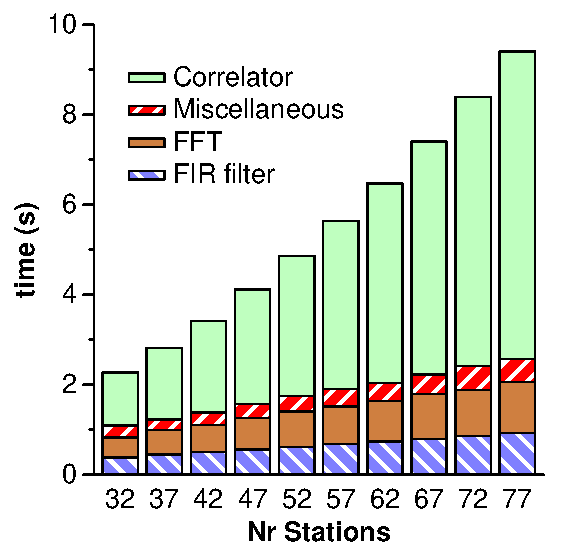
\includegraphics[width=53mm]{speed.eps}
\end{center}
\caption{Execution times to process one second of subband data on one
processor core, for different numbers of stations.  Multiple cores are
necessary to process one subband in real time; consecutive seconds of subband
data are round-robin distributed over the cores.}
\label{fig:speed}
\end{figure}

After the phase correction, the data are correlated, by multiplying the
samples of each station with the complex conjugate of all other stations.
To reduce the output data rate, the correlations are typically integrated
over one second.
Since the cross correlation of station $A$ and $B$ is the complex conjugate
of station $B$ and $A$, only the former is computed.
Autocorrelations are computed as well, but treated separately since they
require only half the amount of computations.
The computational requirements of the correlator grow quadratically with the
number of stations, and dominate the total online processing demands (see
Figure~\ref{fig:speed}).
The correlator, which is also implemented in assembly, is extremely efficient:
it achieves 98\% of the floating-point peak performance~\cite{Romein:06}.

The correlated data are sent to another cluster, the storage section, and
are written to disk.
This is where the real-time pipeline ends.
Eventually, the storage section will be able to store about one Petabyte of
data, so that after an observation, several days are available to calibrate
and image the data.

%Although the BG/L is computationally very efficient,
%streaming the station data into the machine at the required data rates
%turned out to be a major problem,
%despite the BG/L's atypical high number of I/O interfaces.
%For each 16~BG/L compute cores, there is one {\em I/O~node\/} that
%has one external gigabit-Ethernet interface and transparently handles all I/O
%calls initiated by its associated compute cores (see Figure~\ref{fig:IOnode}).
%We found that the stock network system software was not particularly optimized
%for high-throughput I/O, and that the obtained bandwidths were far from what
%theoretically should be achievable.

%The dissatisfaction about the performance and about the I/O model in general
%led to a joint effort to redesign the entire network software infrastructure,
%and resulted in a new environment called {\em ZOID\/}~\cite{Iskra:08}.
%ZOID does not only yield better performance, but it is much more flexible,
%since it allows application code to be run on the I/O~node.
%With ZOID, we were able to move the receipt of the station data from the input
%cluster nodes to the BG/L I/O~nodes, so that the station data are sent
%directly through the WAN into the BG/L.
%Not having to build a separate input cluster results in an estimated cost
%saving of \euro700,000.

\section{Central processing: calibration}

With LOFAR, calibration for radio astronomical instruments enters a new regime. The offline processing has to deal with a number of challenges~\cite{Noordam:04,Noordam:06,Nijboer:07}. First of all, the data volumes are huge. A typical observation in imaging mode produces tens of Tbytes of correlated data. Second, compared to traditional steel dishes, the phased array station beams are far more variable (in time, in frequency, as well as over the different stations), they have a high degree of instrumental polarization that varies with scan angle, and they have relatively high sidelobes. All these issues complicate the processing of the data, especially since a high dynamic range must be reached. 

The third category of challenges lies in the sky itself. At the low frequencies where LOFAR observes there are very bright sources so that a high dynamic range and, hence, a high accuracy is needed to see the faint background sources. The sky will also be filled with a large number of sources, giving rise to confusion. Last, but not least, the Earths ionosphere seriously defocusses the images.

These challenges imply that for LOFAR existing processing strategies and algorithms must be reconsidered and new strategies and algorithms have to be developed. Therefore, the LOFAR offline processing is still a work in progress of which the current status is presented here.

Note: in the radio astronomical community a correlated data sample is called a visibility and it is measured on a baseline: the vector between the two station locations from which the two signals that are correlated originate.
\label{sec:offline}

\subsection{Processing large data volumes}

The total amount of data that is produced is determined by the total number of stations that are used in the observation. This number depends on the particular mode of observation. The correlator produces a data stream of the order of a few Gbyte/s, which yields of the order of several tens of Tbytes of data after a typical observation of four hours. Since a permanent data storage is not part of the LOFAR telescope these data volumes have to be processed near real time. Fortunately, the non-imaging LOFAR applications are not so data intense, so that for every 1 hour of observation approximately 4 hours are available to further process the data offline. With this in mind data I/O becomes an issue. Obviously the data needs to be processed in a parallelized and distributed way minimizing the I/O that is needed~\cite{Loose:08,Diepen:08}.  
 
Data can be distributed over a large number of processing nodes in a number of ways. Distribution over baselines is not very suitable for imaging, where data from all baselines must be combined to produce an image. Distribution over time has the disadvantage that up to several Gbytes/s have to be sent to a single processing node. Frequency, therefore, seems to be the best way. This distribution scheme matches with the design of the correlator. It is also a convenient scheme for the imager, where images are created per (combined) frequency channel.

A consequence of distribution over frequency is that in the self-calibration step solver equations from different compute nodes may need to be combined allowing estimation of parameters using data that is distributed over several nodes. The combining of solver equations, however, involves far less data I/O then the underlying observed visibility data.   

Even though the processing of the data will be done on a large cluster of computers, the total amount of data can be such that the quality of the final result is expected to be processing limited. This means that for all the algorithms accuracy has to be weighted against the amount of FLOPS needed. It also means that the LOFAR instrument can be improved by upgrading the processing cluster in the future. 

\subsection{Processing steps}

LOFAR calibration is a joint estimation problem for both instrumental parameters, environmental (e.g. ionospheric) parameters, and parameters for celestial sources. At its heart lies the ``Measurement Equation'' that is used to model the observed data~\cite{Hamaker:96}. A detailed description of all steps involved can be found in~\cite{Noordam:06}. A signal processing data model and a Cramer-Rao lower bound analysis are given in~\cite{Tol:07}. The latter paper also provides a good introduction to the signal processing aspects of LOFAR calibration.   

\label{sec:RFI}
The current LOFAR calibration strategy consists of the following steps. The first step consists of removing bad data points, which are due to e.g. RFI. After this step the contaminating contribution of a couple of very strong sources (like CasA, CygA, TauA, VirA) that enter through the station beam sidelobes needs to be removed. Since modelling the station beam sidelobes is infeasible due to the large number of parameters involved, the combined effect of the sources and the instrumental effects has to be estimated and subtracted from the data. 

Once the interfering signals are removed from the data, the data is further integrated. The final resolution is determined by bandwidth and time-average smearing requirements that follow from the desired FoV and the maximum baseline~\cite{SIRAII:99}. In the frequency direction the data may be reduced by maximal one order of magnitude. In principle the data is also integrated along the time axis. Here, however, the effect of the ionosphere has to remain constant over the integration period. The maximal reduction factor determined by time-average smearing is also maximally one order of magnitude.

The remaining calibration steps are performed iteratively in a process called
the ``Major Cycle''.
First, the instrumental parameters, the environmental parameters, and parameters for the
brightest celestial sources are estimated, using the visibility data.
Then, after the brightests sources are removed from the visibility data, an
image is constructed. Finally, the parameters of the faint celestial sources are estimated using the image data.
Since not all parameters are estimated jointly, the Major Cycle will be traversed a number of times in order to iteratively refine the estimates~\cite{Noordam:06,Nijboer:07}. 

After initial operation of the LOFAR instrument the parameters for the strongest sources will be known. From then on the strongest sources in the FoV can be used to estimate ionospheric parameters, instrumental parameters, and to refine the estimate for the station beams that is available from the station calibration. It is the direction dependent estimation of ionospheric parameters that is the most challenging part of this estimation problem. 

In~\cite{Tol:07} it is shown that the unconstrained direction dependent calibration problem is ambiguous. However, three physical constraints to get an unambiguous solution are presented: 
%
\begin{enumerate}
\item use a calibrated subarray to calibrate the rest of the array,
\item use assumptions on the structural dependence of a certain corrupting effect, e.g. the ionosphere,
\item use polynomial smoothing on larger time / frequency domains.
\end{enumerate}
% 

In the first approach the LOFAR core is calibrated first, where use is made of the fact that the core stations all share the same ionosphere. This is a simpler problem. Van der Tol {\it et al.}~\cite{Tol:07,Tol:05} show that in this case the remote stations can be calibrated, provided the number of independent calibration directions is less then the number of core stations. 

In the second approach, use is made of the fact that the effect of the ionosphere has a predictable frequency dependence~\cite{Tol:05}. The number of parameters that need to be estimated may be further reduced by using suitable base functions for the spatial dependence of the ionosphere. The use of Karhunen-Loeve base functions seems very promising in this respect~\cite{Tol2:07}.  

In the third approach, multiple samples in frequency and time are combined in a joint estimation, where the time and frequency dependence is modelled by e.g. polynomials and in this way the number of parameters that need to be estimated is reduced from 1 per individual sample to the polynomial coefficients for all samples together. Here use can be made from prior knowledge that not all parameters vary on the same time and frequency scales. In~\cite{Tol:07} it is reported however that this approach needs good initial estimates, since for instance the continuous phase polynomial is ambiguous to integer multiples of $2\pi$.

The sky image is the Fourier transform of the visibility domain. Due to the fact that the visibility domain is only discretely sampled, sources in the sky image are convolved with a Point Spread Function (PSF). The contribution from sources that have PSF far sidelobes that are higher than the image noise level should be subtracted from the visibility data in order to improve the dynamic range of the image. Using the solutions to the parameter estimation problem the contributions from the strongest sources in the FoV are removed from the visibility data. The remaining residual visibility data is then corrected and imaged.

One visibility sample contains the combined contribution from all sources in the sky. Since LOFAR has a large FoV, the contribution from different sources is distorted by different ionospheric and beam effects. When imaging the visibility data, however, it is only possible to correct the data for one direction in the sky. This would mean that the image would be sharp for the direction of correction and the image quality would degrade outwards. To overcome this problem LOFAR images will be made in small facets, where the data can be corrected for the center of each facet. 

Facet imaging is a well known technique to overcome smearing effects that are due to the fact that the baselines are non-coplanar~\cite{SIRAII:99}. However, the non-coplanar baseline problem is better solved by the w-projection algorithm~\cite{Cornwell:05}. Applying the w-projection technique per facet ensures that the maximum facet size is not restricted by the effect of the non-coplanar baselines, but the facet size will only be determined by the variability of the station beam and the ionosphere.

The facet size is far smaller then the total FoV, which allows the data to be further integrated in both time and frequency. However, since for every facet a new set of integrated, corrected data is constructed the total amount of data will be approximately the same as the full resolution, observed data.
  
Once the image is produced, source finding and source extraction algorithms will be used to estimate source parameters for the faint sources and refine the parameter estimates for the bright sources. This results in an updated source model and a new cycle of the Major Cycle is entered. 

\section{Current state and future work}

\subsection{Core Station 1}
Currently, four partially-built stations, also referred to as Core Station~1
(CS1), are functional~\cite{gunst:06}.
One of those stations contains the hardware to observe with 48~LBAs or with
6~HBA tiles and 30~HBA elements. Figure~\ref{fig:cs1} shows the LBA field of this station.

\begin{figure}
\begin{center}
\includegraphics[width=.5\columnwidth]{cs1photo.eps}
\end{center}
\caption{Picture of the LBA antenna field at one of the stations.}
\label{fig:cs1}
\end{figure}

The other 3~stations are equipped with 16~LBAs and 4~HBA elements each.
To create more baselines and achieve better spatial coverage, all stations
can be split into four {\em microstations}.
This yields 16~microstations, which are treated the same as real stations in
the online and offline processing pipelines.

%A consequence of quadrupling the number of stations is that the bandwidth
%is reduced to 36~subbands of 195~kHz or 48~subbands of 156~kHz.
%Alternatively, the station with 48~LBA can be split into 12~microstations,
%so that together with the other $3\times4$ microstations a total of
%24~microstations can be formed. Currently WAN restrictions limit the bandwidth to 12~resp.\ 16~subbands.

The WAN infrastructure from the field towards the central location is realized for all four stations. At the central location, part of the input cluster and offline cluster are built, to match with the data streams coming from the field. These clusters will be scaled up when more stations become available. Six BG/L racks are available for the main part of the online processing. The BG/L is capable of handling all foreseen future data rates.

Many LBA commissioning observations have been done so far. The development of the HBA was finished last year and the commissioning of the HBA tiles is still ongoing. Currently all the equipment in the field is operational.

Figure \ref{fig:skymap} shows a series of images that were made from data using CS1~\cite{Yatawatta:08}. In total 16~microstations, each consisting of a single dipole with essentially an all sky FoV, were used. The images are centered on the North Celestial Pole and contain 48 hours and about 20 subbands of data. First the data is flagged for RFI and an image of the flagged-only data is shown on the left (``observed''). 

\begin{figure*}
\centering
\includegraphics[width=0.32\textwidth]{LBA_observed.eps}
\includegraphics[width=0.32\textwidth]{LBA_calibrated.eps}
\includegraphics[width=0.32\textwidth]{LBA_peeled.eps}
\caption{All sky images from the LOFAR CS1 configuration using 48 hours and about 20 subbands of data. Observed: an image of the flagged, non-calibrated data. Calibrated: an image of the flagged, calibrated data showing CasA and CygA. Residual: an image of the flagged, calibrated data where CasA and CygA are removed from the data. Images courtesy of S.B. Yatawatta.}
\label{fig:skymap}
\end{figure*}

Calibration is performed in two steps. In the first step, a point source model is used for both CasA and CygA, both at 20000 Jy flux and no polarization. An analytical beam shape is used and a single complex gain per station for the whole sky is estimated. In this way an estimate for the instrumental complex gains (e.g. due to clock drifts) and ionospheric phase differences is obtained. After correcting the data, a second step is performed where the complex gains in both the direction of CasA and CygA are estimated. In this second step no assumptions on the beam are made. For the middle image (``calibrated'') the data is corrected using the estimates for the direction of CasA. In this middle image CasA and CygA can be clearly seen as point sources. 

CasA and CygA completely dominate the background sources, since they are at least 50 times stronger then the strongest background source. After subtracting the contributions from CasA and CygA from the data some 100 other sources become visible. This is shown in the right panel (``residual''). 

\subsection{International stations}
There is a growing international interest in building stations outside the
Netherlands.
With these stations, longer baselines can be established.
The first international station, consisting of 96~LBA antennas, is currently
operational in Effelsberg (Germany) and will be connected to the central
processor soon.
Two additional German stations will be installed in Garching and Tautenburg.
More stations are planned in Germany (Potsdam), Sweden, France, and the
United Kingdom, and interest is shown by Poland and Italy.
The international stations can operate in stand-alone mode or participate
in the full LOFAR configuration.

\subsection{Scaling LOFAR}
In the course of this year, 18~stations will be manufactured and installed in the field. Also, the WAN infrastructure and central processor facility will be scaled up to handle the data from the 18 stations and the international stations.
The remainder of the stations will be built in 2009.

The software development currently focusses on the imaging mode.
In the course of this year significant effort will be put in realizing the
tied-array beamforming mode.


% if have a single appendix:
%\appendix[Proof of the Zonklar Equations]
% or
%\appendix  % for no appendix heading
% do not use \section anymore after \appendix, only \section*
% is possibly needed

% use appendices with more than one appendix
% then use \section to start each appendix
% you must declare a \section before using any
% \subsection or using \label (\appendices by itself
% starts a section numbered zero.)
%


%\appendices
%\section{Proof of the First Zonklar Equation}
%Appendix one text goes here.

% you can choose not to have a title for an appendix
% if you want by leaving the argument blank
\section{}
%Appendix two text goes here.


% use section* for acknowledgement
\section*{Acknowledgment}


This work reflects the effort of the whole LOFAR team.

LOFAR is funded by the Dutch government in the BSIK programme for
interdisciplinary research for improvements of the knowledge infrastructure.
Additional funding is provided by the European Union, European Regional
Development Fund (EFRO) and by the ``Samenwerkingsverband Noord-Nederland,''
EZ/KOMPAS.

ASTRON is part of the Netherlands Foundation for Scientific Research, NWO.

% Can use something like this to put references on a page
% by themselves when using endfloat and the captionsoff option.
\ifCLASSOPTIONcaptionsoff
  \newpage
\fi



% trigger a \newpage just before the given reference
% number - used to balance the columns on the last page
% adjust value as needed - may need to be readjusted if
% the document is modified later
%\IEEEtriggeratref{8}
% The "triggered" command can be changed if desired:
%\IEEEtriggercmd{\enlargethispage{-5in}}

% references section

% can use a bibliography generated by BibTeX as a .bbl file
% BibTeX documentation can be easily obtained at:
% http://www.ctan.org/tex-archive/biblio/bibtex/contrib/doc/
% The IEEEtran BibTeX style support page is at:
% http://www.michaelshell.org/tex/ieeetran/bibtex/
%\bibliographystyle{IEEEtran}
% argument is your BibTeX string definitions and bibliography database(s)
%\bibliography{IEEEabrv,../bib/paper}
%
% <OR> manually copy in the resultant .bbl file
% set second argument of \begin to the number of references
% (used to reserve space for the reference number labels box)
%\begin{thebibliography}{1}
%
%\bibitem{IEEEhowto:kopka}
%H.~Kopka and P.~W. Daly, \emph{A Guide to \LaTeX}, 3rd~ed.\hskip 1em plus
%  0.5em minus 0.4em\relax Harlow, England: Addison-Wesley, 1999.
%
%\end{thebibliography}
\bibliographystyle{IEEEtran}
\bibliography{lofar,lofarRJN}

% biography section
% 
% If you have an EPS/PDF photo (graphicx package needed) extra braces are
% needed around the contents of the optional argument to biography to prevent
% the LaTeX parser from getting confused when it sees the complicated
% \includegraphics command within an optional argument. (You could create
% your own custom macro containing the \includegraphics command to make things
% simpler here.)
%\begin{biography}[{\includegraphics[width=1in,height=1.25in,clip,keepaspectratio]{mshell}}]{Michael Shell}
% or if you just want to reserve a space for a photo:

\begin{IEEEbiography}[{\includegraphics[width=1in,height=1.25in,clip,keepaspectratio]{gunst.eps}}]{Andr\'{e} W. Gunst}
is a digital system engineer at ASTRON and currently responsible for the development of the LOFAR system. He obtained a degree in Electrical Engineering from Twente University, Enschede, the Netherlands in 1999. Since, 2004 he worked on the development of the station systems in LOFAR. In 2006 he became responsible for the development of the overall LOFAR system for the astronomical applications. His research interests include (digital) system design and digital signal processing.
\end{IEEEbiography}

\begin{IEEEbiography}[{\includegraphics[width=1in,height=1.25in,clip,keepaspectratio]{rnijboer.eps}}]{Ronald Nijboer}
is leading the Computing group at ASTRON. He obtained a degree in Mathematics from the Eindhoven University of Technology in 1994. His Ph.D. research on waves and instabilities of flowing  plasmas he performed at the FOM Institute for Plasma Physics ``Rijnhuizen''. He received the Ph.D. degree in 1998 from the Vrije Universiteit, Amsterdam. From 1998 till 2004 he worked in the field of aeroacoustics with the National Aerospace Laboratory (NLR). In 2004 he started working for ASTRON. His research interests include calibration and imaging algorithms.  
\end{IEEEbiography}


% if you will not have a photo at all:
%\begin{IEEEbiographynophoto}{John Doe}
%Biography text here.
%\end{IEEEbiographynophoto}

% insert where needed to balance the two columns on the last page with
% biographies
%\newpage

\begin{IEEEbiography}[{\includegraphics[width=1in,height=1.25in,clip,keepaspectratio]{romein.eps}}]{John W.\ Romein}
is a senior system engineer/researcher high-performance
computing at ASTRON, where he is responsible for the online data processing
of LOFAR.
He obtained his Ph.D.\ on distributed board-game playing at the Vrije
Universiteit, Amsterdam.
As a postdoc, he solved the game of Awari using a large computer cluster,
and did research on parallel algorithms for bio-informatics.
His research interests include high-performance computing, parallel algorithms,
networks, programming languages, and compiler construction.
\end{IEEEbiography}
%\end{IEEEbiographynophoto}

% You can push biographies down or up by placing
% a \vfill before or after them. The appropriate
% use of \vfill depends on what kind of text is
% on the last page and whether or not the columns
% are being equalized.

%\vfill

% Can be used to pull up biographies so that the bottom of the last one
% is flush with the other column.
%\enlargethispage{-5in}



% that's all folks
\end{document}


